% arara: pdflatex
% arara: showfile
\documentclass[border=0pt]{standalone}
\usepackage{tikzlings}
\usetikzlibrary{ducks}
\usetikzlibrary{shapes.geometric}
\definecolor{blueinter}{RGB}{0,102,170}%
\tikzset{
  linea/.style={white, line width=4pt,},
  pics/microph/.style={code={ 
        \draw[black, line width=.2em, rounded corners=1.7ex] 
            (-.85em,4.5ex) -- (-.85em,2ex) -- (.85em,2ex) -- (.85em,4.5ex);
        \fill[black] 
            (-.6em,5ex) to[rounded corners=1.2ex]  
            (-.6em,2.5ex) to[rounded corners=1.2ex] (.6em,2.5ex)
            -- (.6em,5ex) to[rounded corners=.2ex] ++(-.85em,0) to[rounded corners=.2ex] ++(0,.35ex) -- ++(.85em,0)  
            -- (.6em,5.5ex) to[rounded corners=.2ex] ++(-.85em,0) to[rounded corners=.2ex] ++(0,.35ex) -- ++(.85em,0)
            -- (.6em,6ex) to[rounded corners=.2ex] ++(-.85em,0) to[rounded corners=.2ex] ++(0,.35ex) -- ++(.85em,0)
            -- (.6em,6.5ex) to[rounded corners=.2ex] ++(-.85em,0) to[rounded corners=.2ex] ++(0,.35ex) -- ++(.85em,0)
            to[rounded corners=1.2ex]
            (.6em,8ex) to[rounded corners=1.2ex]
            (-.6em,8ex) to cycle; 
    }},
}
\begin{document}
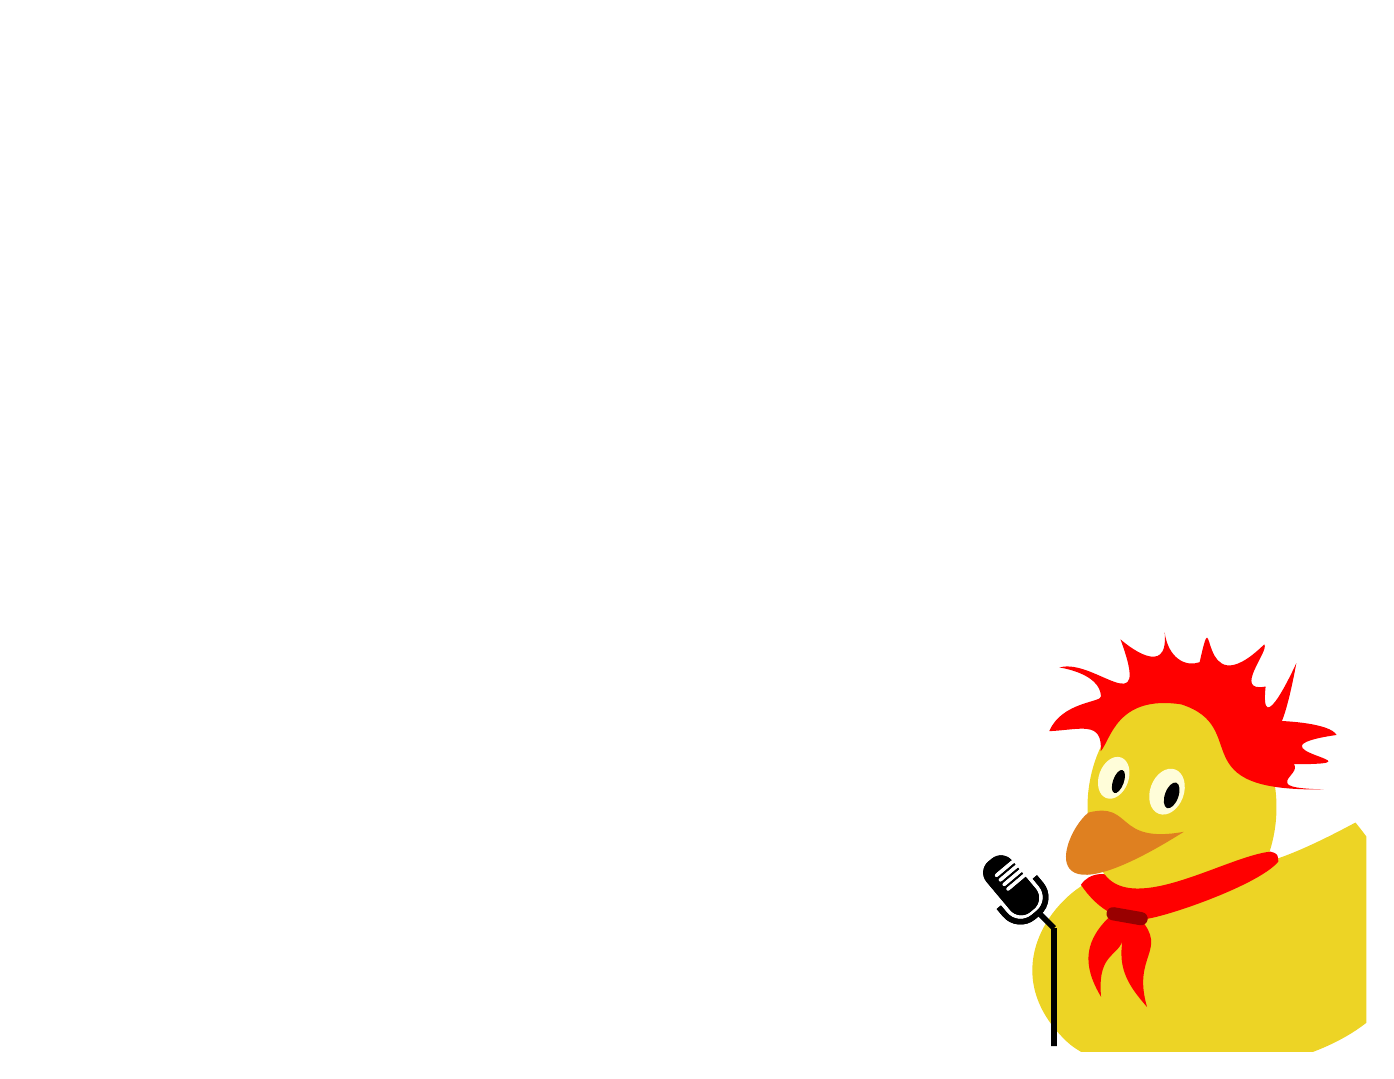
\begin{tikzpicture}
\begin{scope}
\pic[rotate=40, local bounding box=microfono] at (4.5,-5) {microph};
\clip (-8.5,-6.5) rectangle (8.5,6.5);
% background
\node[minimum width=17cm, minimum height=13cm](sky){};
% Gianna 
\pic[scale=2.4,
	duck/neckerchief=red,
	duck/crazyhair=red,
	duck/woggle=red!60!black
	] at (4,-7) {duck};
	\pic[rotate=40] at (4.5,-5) {microph};
	\draw[black, line width=2pt] (microfono.-45) -- ++(-.2,+.2) ++(.2,-.2) -- ++(0,-1.5);
\end{scope}
\end{tikzpicture}
\end{document}